\documentclass[11pt]{article}

\usepackage[margin=1in]{geometry}
\usepackage{parskip}
\usepackage{graphicx}
\usepackage{amsmath}
\usepackage{subcaption}
\usepackage[hidelinks]{hyperref}

\graphicspath{{figures/}}

\title{Pilot study on grokking in RL}
\author{}
\date{\today}

\begin{document}
\maketitle

\section{Overview}

Fernando, David, and I hypothesized that grokking occurs in RL and that it affords better
generalization. This is to say that task performance can plateau while
continued training leads to more abstract belief representation which then
becomes useful when learning a new but related task.
Here, we explored this using decoded belief resolution as a proxy for grokking. Whether it is or not was not explored here.

\section{Initial Training on The First Task}

A single seed is trained, using PPO, to predict the tokens emitted by an HMM.
In a second variant, it is trained with PPO and an auxiliary cross entropy
next token prediction loss.

The process is the Cyclic Pusher HMM, a three state process with a two-token
alphabet, designed by Alec Boyd. Agents have a two-dimensional action space,
each corresponding to one of the tokens in the HMM's alphabet. A reward of 1
is given if the emitted action corresponds to the token emitted by the HMM at
that time step and 0 otherwise.

The second variant uses an additional head that also has a two-dimensional
output on which an NTP cross entropy loss is applied.

The model's belief representation as measured against the true Bayesian
target is measured with a linear probe at each checkpoint.

\subsection{Performance and Representation}

Performance plateaus near optimal while the belief representation improves
for a long period after in Figure~\ref{fig:task1-ppo}
and~\ref{fig:task1-ppo-ce}. The second variant does not improve convergence
time to task competency but does improve representation per training budget.

\subsection{Three Important Checkpoints}

For each of the two training variants, three checkpoints are highlighted. All
three have nearly identical task performance. However, the first checkpoint, A, has
much worse belief resolution (as recovered by the linear probe) compared to
the third checkpoint, C. The second checkpoint, B, of the PPO-only run also
has worse belief resolution but is much improved in the PPO+CE run.

\begin{figure}[p]
  \centering
  \begin{subfigure}{\textwidth}
    \centering
    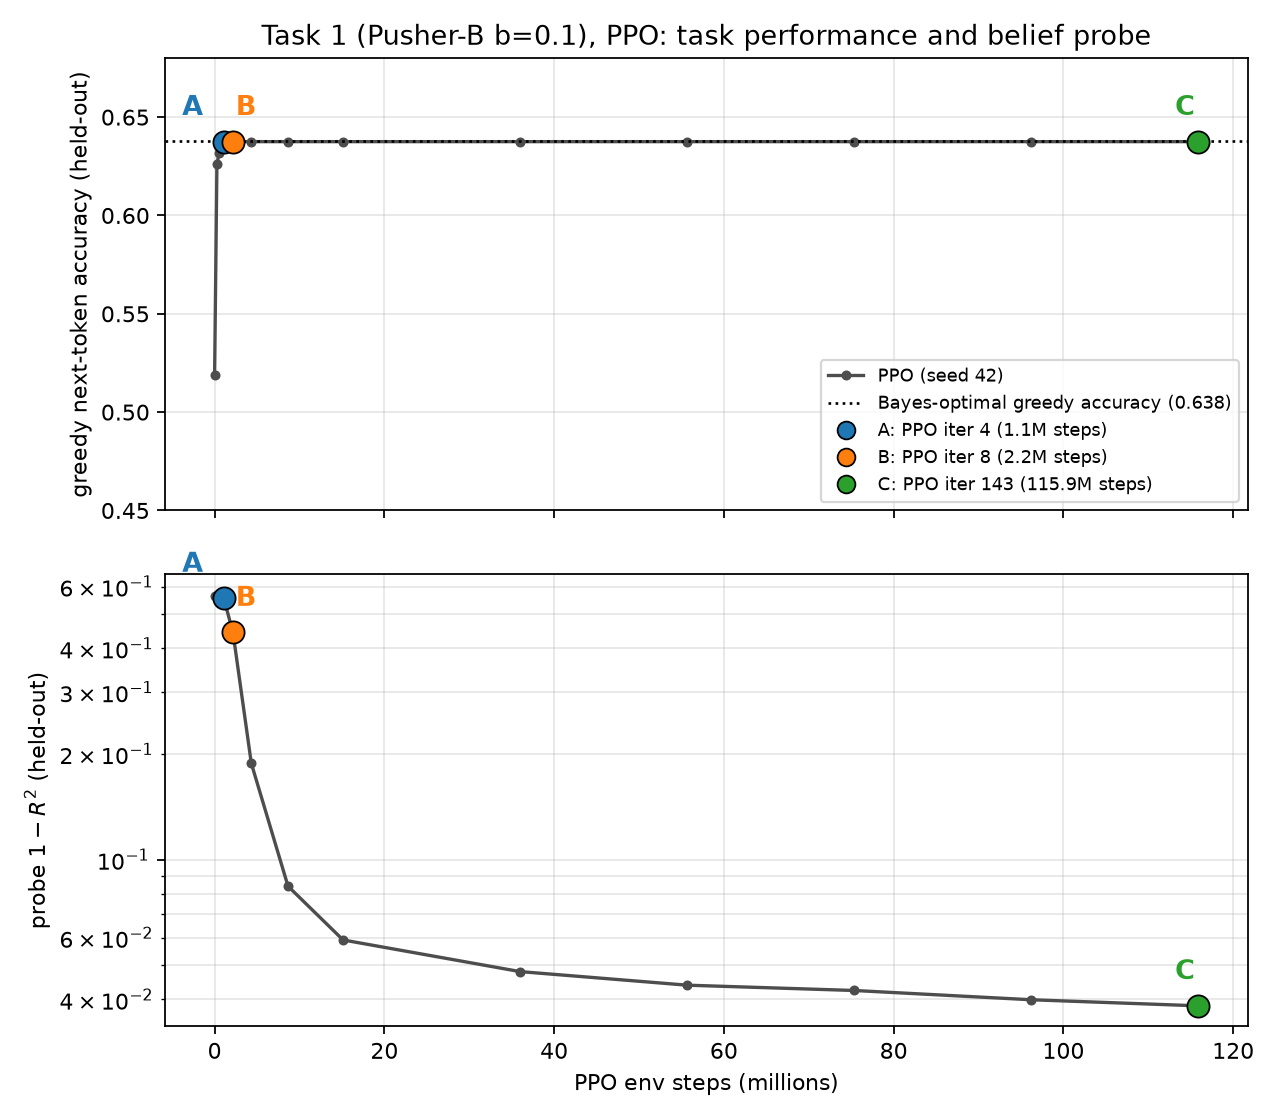
\includegraphics[width=0.65\textwidth]{fig1a_task1_ppo}
    \caption{PPO.}
    \label{fig:task1-ppo}
  \end{subfigure}
  \begin{subfigure}{\textwidth}
    \centering
    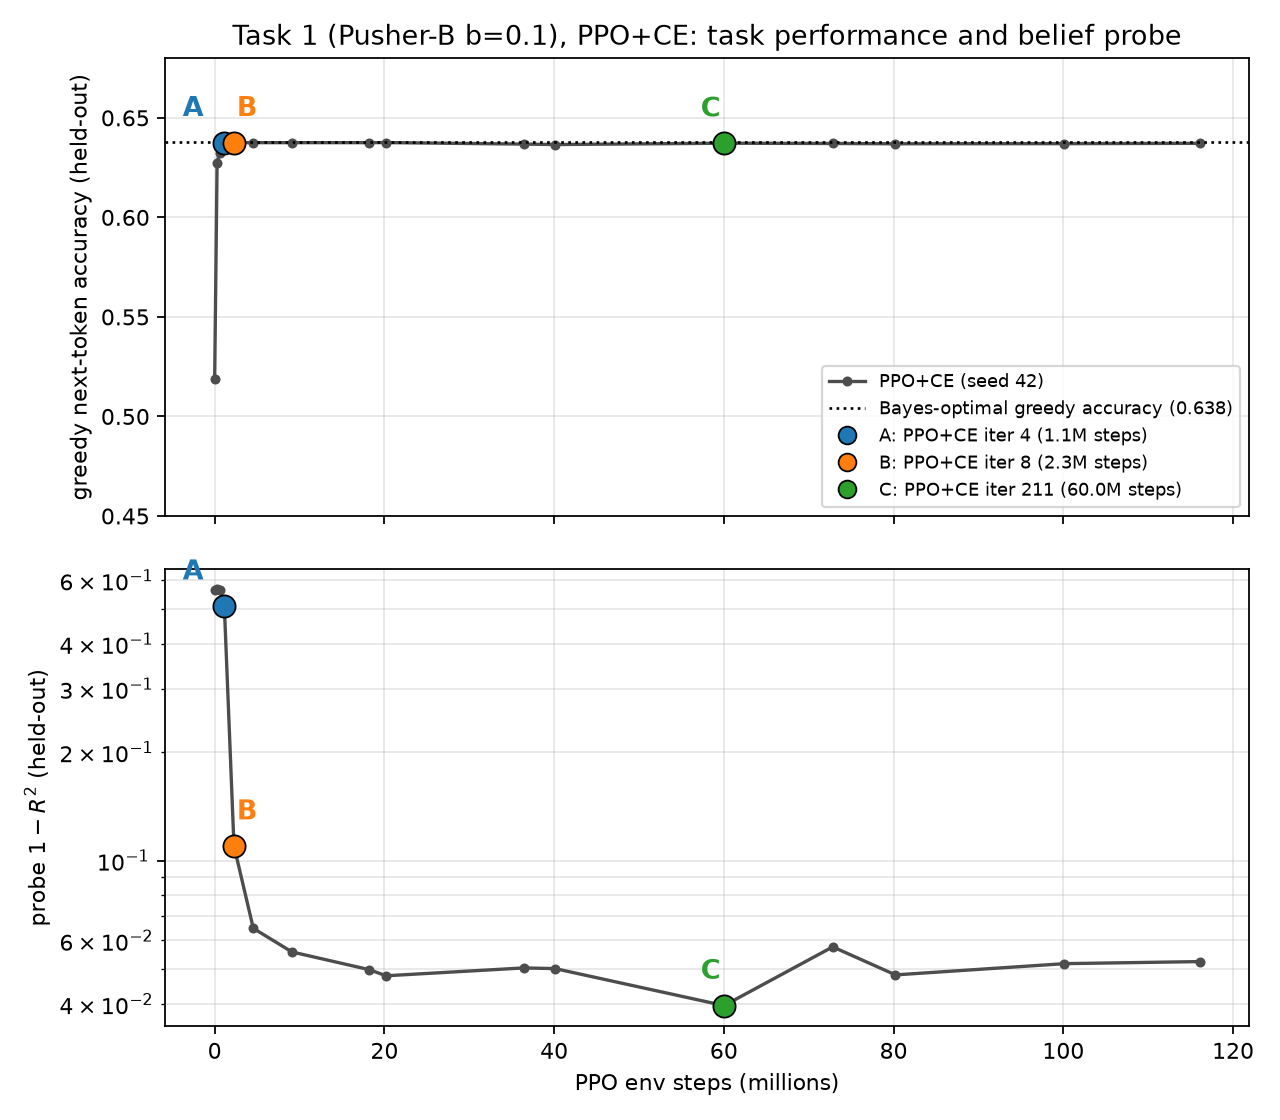
\includegraphics[width=0.65\textwidth]{fig1b_task1_ppo_ce}
    \caption{PPO+CE.}
    \label{fig:task1-ppo-ce}
  \end{subfigure}
  \caption{Held-out greedy accuracy and held-out affine belief-probe
  $1-R^2$ on task 1, with selected checkpoints A, B and C marked.
  Lower $1-R^2$ means better linear decoding. Each panel shows one training run.}
  \label{fig:task1}
\end{figure}

\section{The Second Task}

Each of the checkpoints are then trained on a new task. The second task is the same as the first but we add a third action, pass, with reward $0$, and change the wrong-guess
reward to $-2$; a correct guess still earns $+1$.  If the most likely token has conditional probability $p$,
the expected reward of guessing it is $p-2(1-p)=3p-2$. The Bayes rule is
therefore to guess when $p>2/3$, pass when $p<2/3$, and choose either at
equality. Because actions do not change future observations or dynamics,
there is no information-gathering advantage to guessing.

\subsection{Belief Decodability and Transfer Performance}

As predicted, checkpoints with better belief representation in the first task
do better on the second task ie C beats A even though all checkpoints have the same
performance on the first task ie A, B, and C are equivalent. All checkpoints do better than
one trained from scratch (light gray line). Figure~\ref{fig:task2-full-ppo}.

\begin{figure}[htbp]
  \centering
  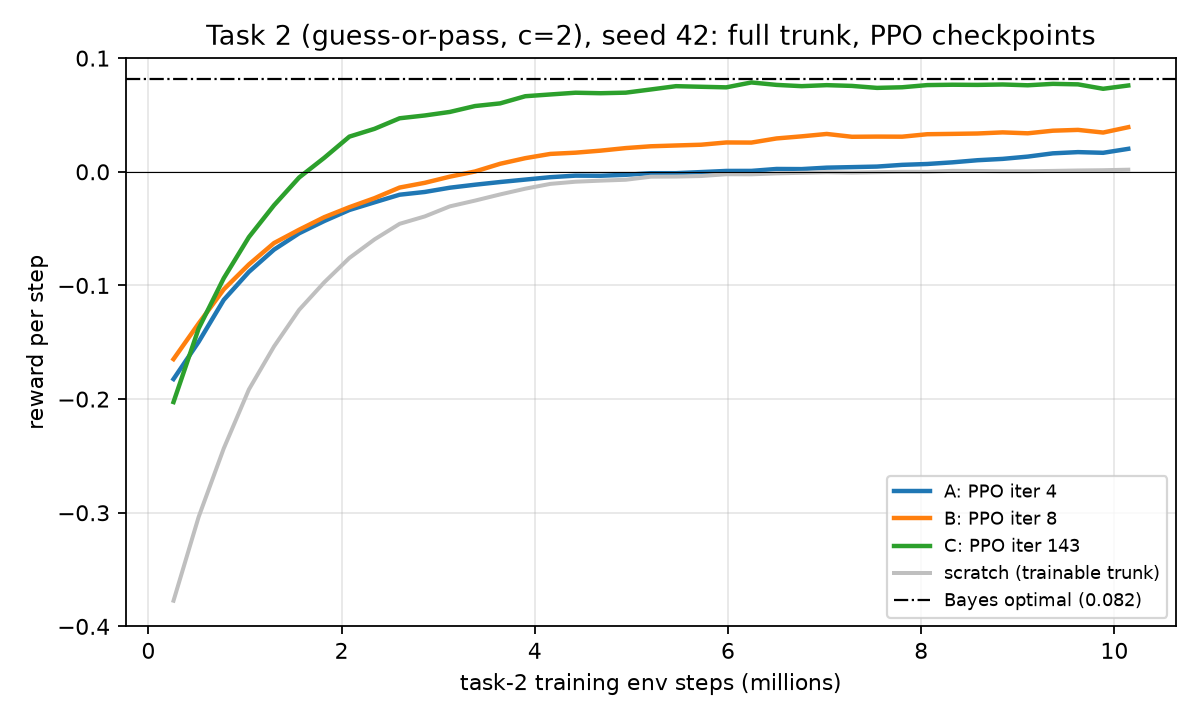
\includegraphics[width=0.85\textwidth]{fig2_full_ppo}
  \caption{PPO-only full-trunk runs on the second task.}
  \label{fig:task2-full-ppo}
\end{figure}

\subsection{The Effect of Better Belief Resolution From A Predictive Loss}

The clearest observed transfer advantage of PPO+CE over PPO occurs at
checkpoint B, where the task-1 belief-probe scores also differ substantially.

Comparing figure~\ref{fig:task1-ppo} to figure~\ref{fig:task1-ppo-ce} shows
that belief decoding improves earlier with cross entropy in these runs.
At checkpoint B, held-out probe $R^2$ is 0.556 for PPO and 0.890 for PPO+CE,
at similar traning step counts.

Figure~\ref{fig:task2-full-ppo-vs-ce} compares the performance of PPO-only
checkpoints to those from PPO+CE on the second task. Performance on the
second task is the same for checkpoints A and C whether or not it was trained
with CE. However, checkpoint B shows better second-task performance when it
has better belief resolution as conferred by CE.

\begin{figure}[htbp]
  \centering
  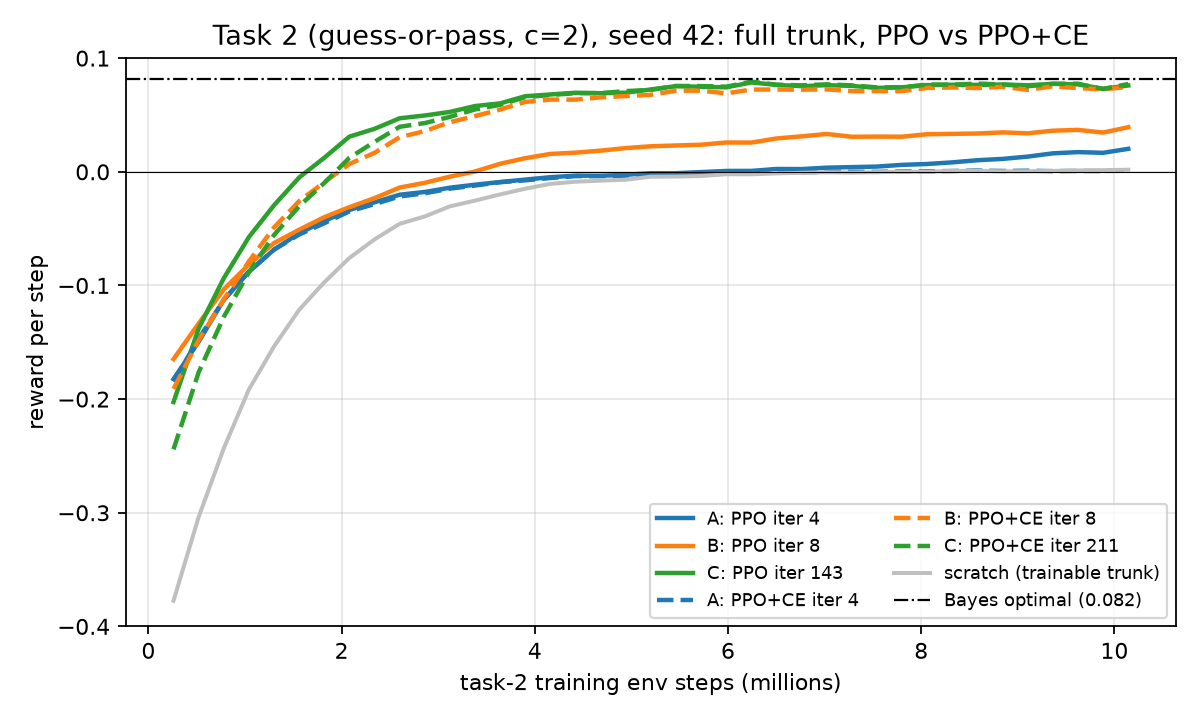
\includegraphics[width=0.85\textwidth]{fig3_full_ppo_vs_ppo_ce}
  \caption{Full-trunk PPO-only runs plus PPO+CE runs on the second task. Checkpoint B is the only one where PPO+CE provides a transfer advantage and is also the only one where the belief representation is better resolved (when comparing checkpoint to checkpoint from PPO-only vs PPO+CE).}
  \label{fig:task2-full-ppo-vs-ce}
\end{figure}

\subsection{Freezing The Trunk}

Testing on a frozen trunk made learning the second task more difficult but
still preserved the ranking of the three checkpoints
(Figure~\ref{fig:task2-frozen-ppo} and~\ref{fig:task2-frozen-ppo-ce}) with the
exception of the comparison between PPO-only and PPO+CE on checkpoint B.

\begin{figure}[p]
  \centering
  \begin{subfigure}{\textwidth}
    \centering
    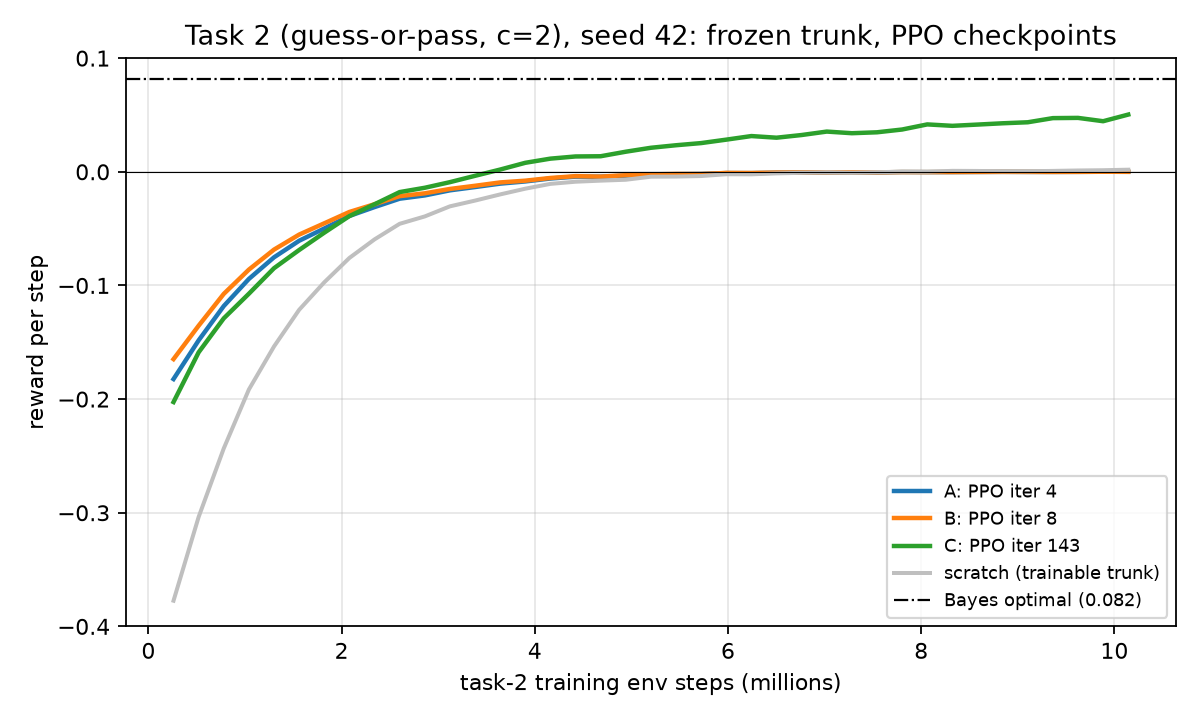
\includegraphics[width=0.85\textwidth]{fig4a_frozen_ppo}
    \caption{PPO-only.}
    \label{fig:task2-frozen-ppo}
  \end{subfigure}
  \begin{subfigure}{\textwidth}
    \centering
    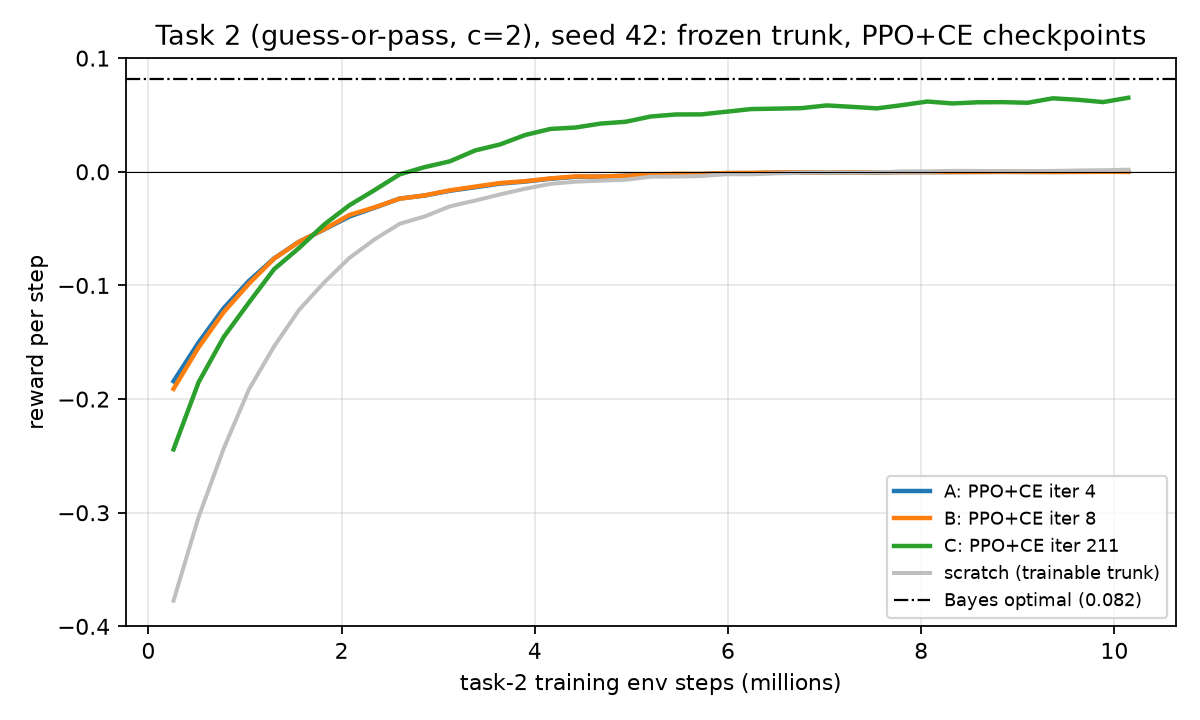
\includegraphics[width=0.85\textwidth]{fig4b_frozen_ppo_ce}
    \caption{PPO+CE.}
    \label{fig:task2-frozen-ppo-ce}
  \end{subfigure}
  \caption{Frozen-trunk runs on the second task.}
  \label{fig:task2-frozen}
\end{figure}

\section{Confounds}

The later checkpoint performing better on the new task could be the result of
factors other than grokking since it has more experience. A better test would
be to use off-policy RL on a small-enough set of experience.

Working against the older checkpoints, however, is loss of plasticity
typically seen in late-training such as from constant neurons.

\end{document}
